\documentclass[tikz,border=3pt]{standalone}
\usepackage[utf8]{inputenc}
\usepackage[T1]{fontenc}
\usepackage{lmodern}
\renewcommand{\familydefault}{\sfdefault}
\usepackage{sansmath}\sansmath
\usepackage{chemfig}
\usepackage{pgfplots}\pgfplotsset{compat=1.18,/pgf/number format/use comma,/pgf/number format/1000 sep={.}}
\usetikzlibrary{arrows.meta,calc,positioning,decorations.pathmorphing,patterns}
% paleta del sitio
\definecolor{nar}{HTML}{E8680C}\definecolor{narc}{HTML}{FFB35C}\definecolor{hielo}{HTML}{FFF3E8}
\definecolor{tinta}{HTML}{1D1D1F}\definecolor{gris}{HTML}{6E6E73}\definecolor{lila}{HTML}{7C5CF0}
\definecolor{azul}{HTML}{2F6FD6}\definecolor{menta}{HTML}{17A673}\definecolor{coral}{HTML}{E8342A}
\begin{document}
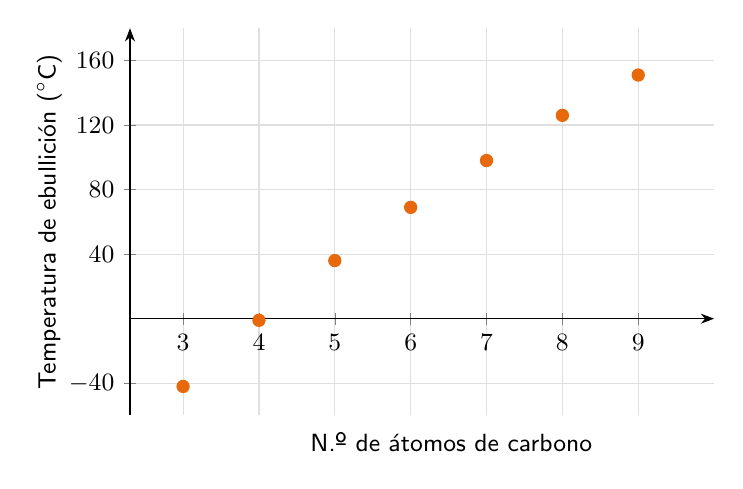
\begin{tikzpicture}[font=\small]
\begin{axis}[width=9cm,height=6.5cm,axis lines=middle,xmin=2.3,xmax=10,ymin=-60,ymax=180,xtick={3,4,5,6,7,8,9},ytick={-40,0,40,80,120,160},
  grid=major,grid style={gray!25},xlabel={N.º de átomos de carbono},ylabel={Temperatura de ebullición ($^\circ$C)},
  xlabel style={at={(axis description cs:0.55,-0.02)},anchor=north},ylabel style={rotate=90,at={(axis description cs:-0.1,0.5)},anchor=south},
  x axis line style={-{Stealth}},y axis line style={-{Stealth}}]
\addplot[only marks,mark=*,mark options={fill=nar,draw=nar,scale=1.1}] coordinates {(3,-42)(4,-1)(5,36)(6,69)(7,98)(8,126)(9,151)};
\node[anchor=east,font=\small] at (axis cs:2.3,0) {0};
\end{axis}
\end{tikzpicture}
\end{document}
